\appendix
\chapter{Figures and Tables}
%Information typically included are things like program listings, complex circuit diagrams, tables, proofs, graphs or any other material which would break up the theme of the text.

%!!!!!!!!!!!!!!!!put a small introduction on what will the reader see in this appendix

\begin{figure}[H]
\centering
\subfigure[RGB raw image]{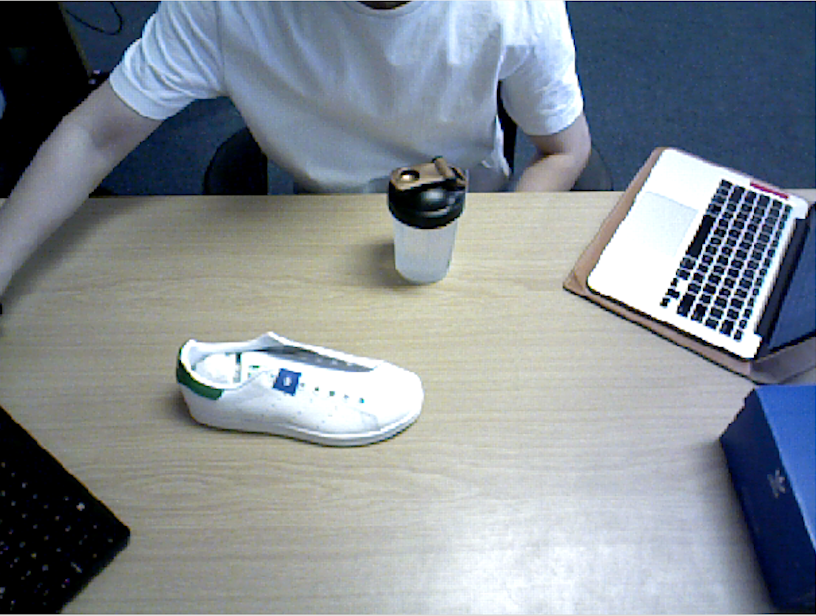
\includegraphics[width = 0.45\columnwidth]{Implementation/cv/raw.png}}
\subfigure[YOLO detection image including bounding boxes]{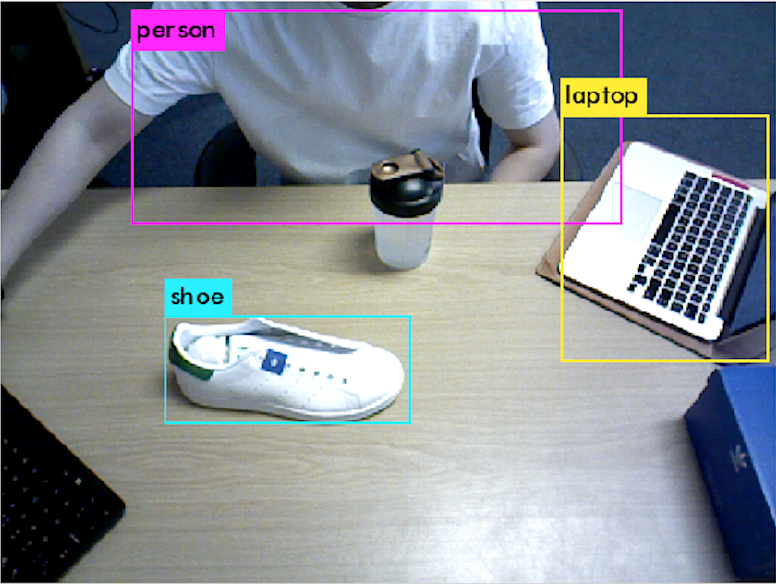
\includegraphics[width = 0.45\columnwidth]{Implementation/cv/yolo.png}}
\caption{ASUS Xtion camera image before and after using YOLO detection system}
\label{5.2asus}
\end{figure}

\begin{figure}[H]
\centering
\subfigure[RGB raw image]{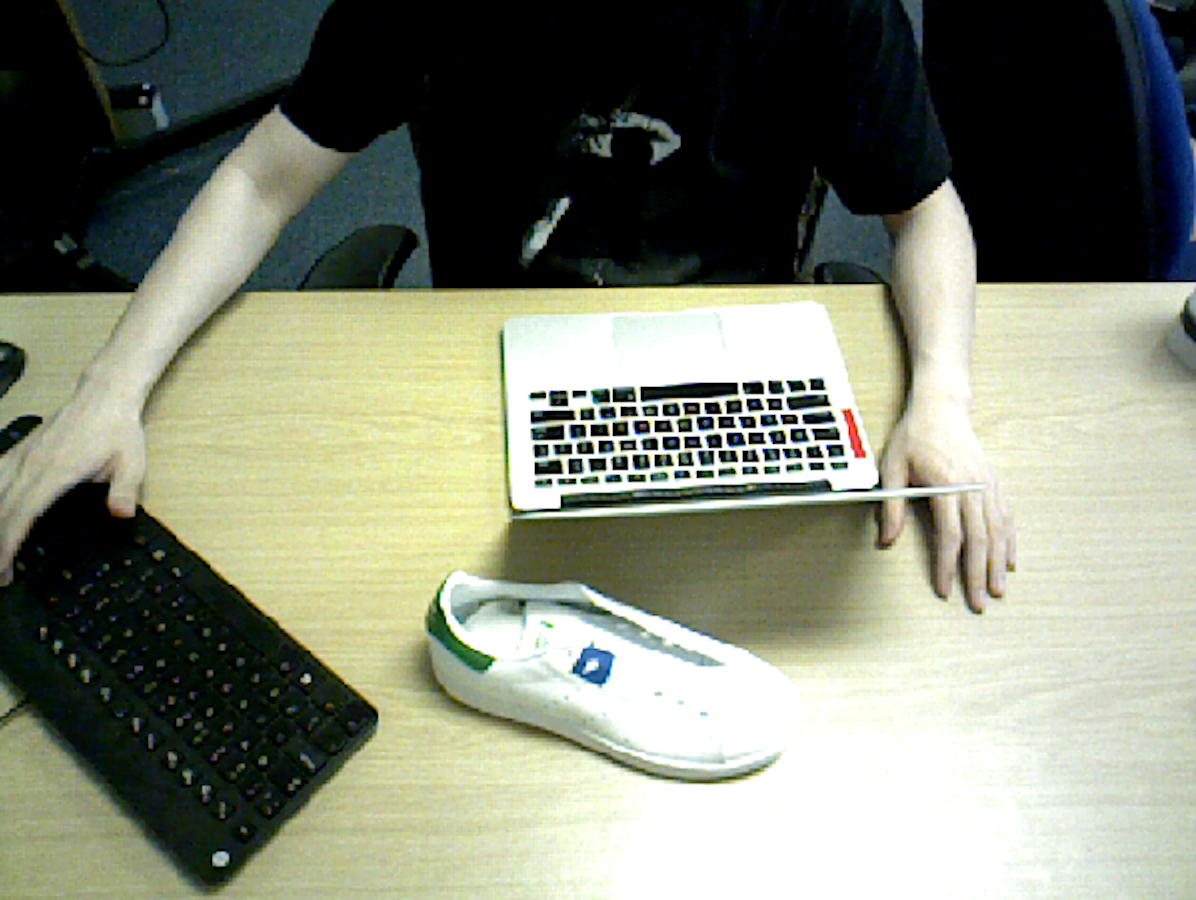
\includegraphics[height=5cm,keepaspectratio]{Implementation/cv/rgbpt.png}}
\subfigure[Depth registered point clouds]{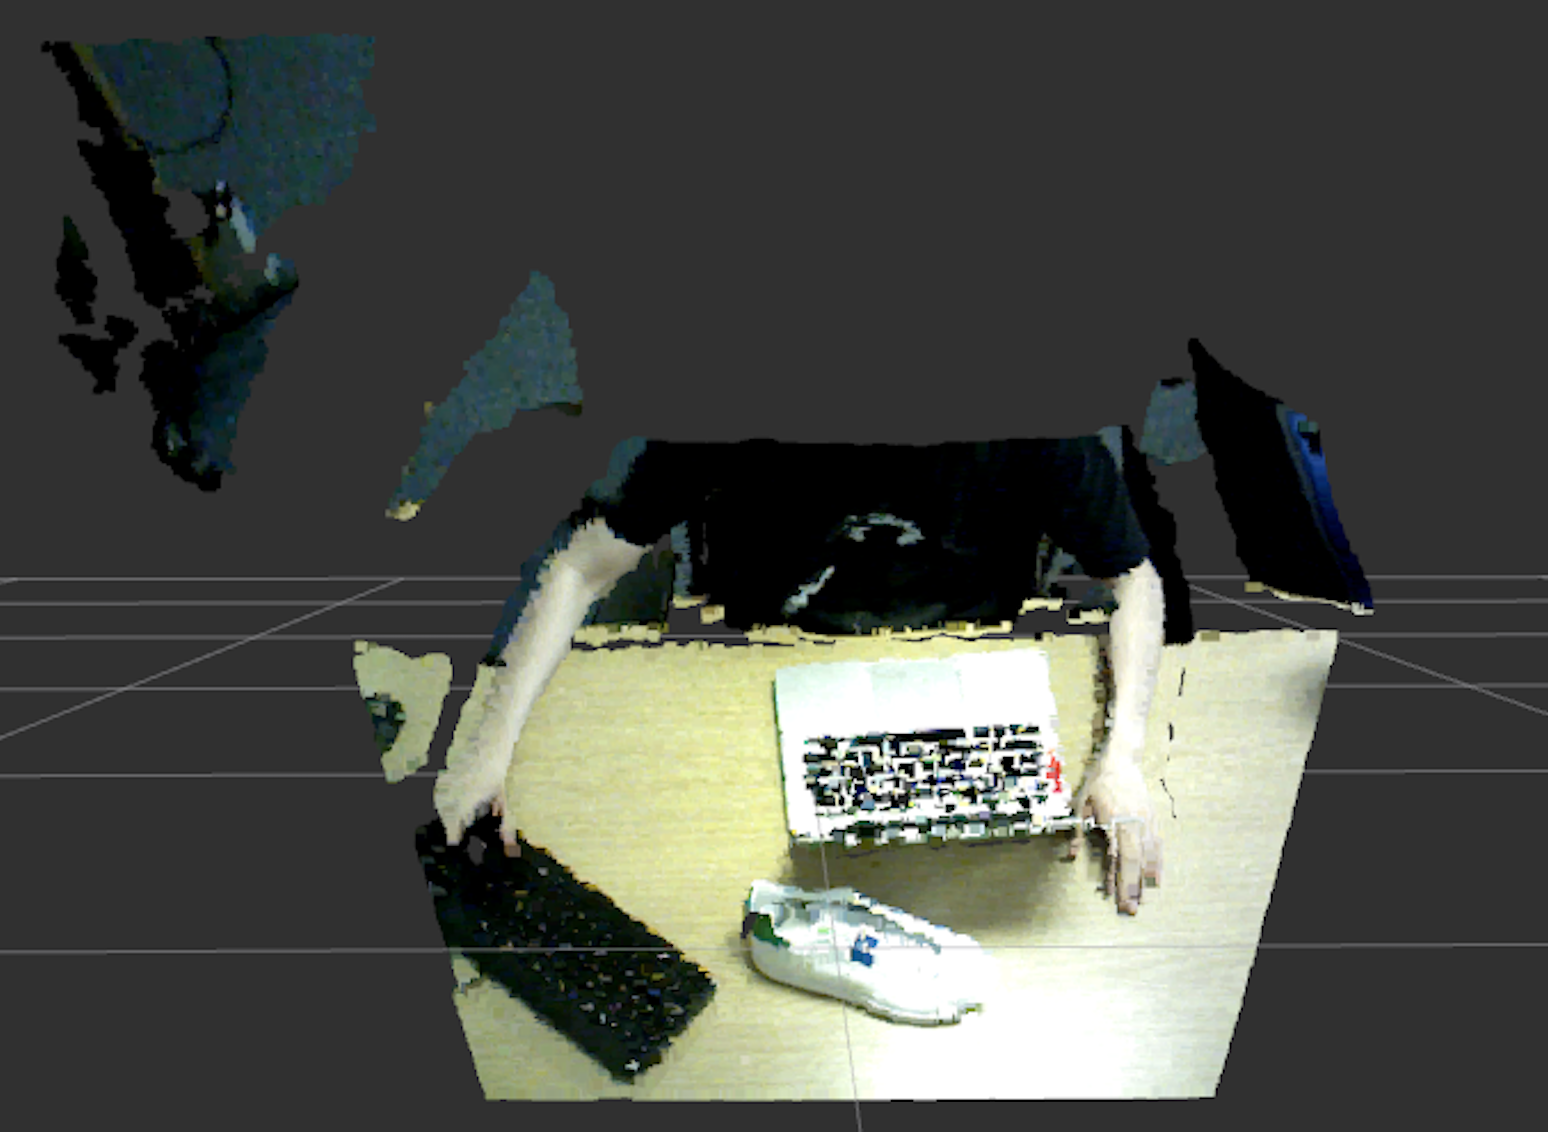
\includegraphics[height=5cm,keepaspectratio]{Implementation/cv/ptcloud.png} \label{ptcloud}}
\caption{Messages of different ASUS Xtion camera topics}
\end{figure}

\begin{figure}[H]
\centering
\subfigure{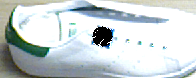
\includegraphics[width = 0.24\columnwidth]{Implementation/cv/bi1.png}}
\subfigure{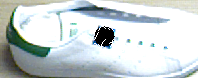
\includegraphics[width = 0.24\columnwidth]{Implementation/cv/g1.png}}
\subfigure{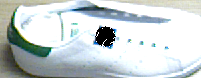
\includegraphics[width = 0.24\columnwidth]{Implementation/cv/m1.png}}
\subfigure{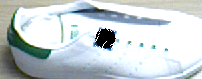
\includegraphics[width = 0.24\columnwidth]{Implementation/cv/b1.png}}

\subfigure{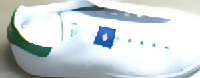
\includegraphics[width = 0.24\columnwidth]{Implementation/cv/bi2.png}}
\subfigure{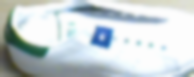
\includegraphics[width = 0.24\columnwidth]{Implementation/cv/g2.png}}
\subfigure{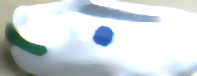
\includegraphics[width = 0.24\columnwidth]{Implementation/cv/m2.png}}
\subfigure{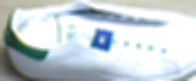
\includegraphics[width = 0.24\columnwidth]{Implementation/cv/b2.png}}

\subfigure{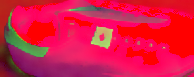
\includegraphics[width = 0.24\columnwidth]{Implementation/cv/bi3.png}}
\subfigure{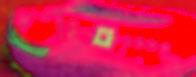
\includegraphics[width = 0.24\columnwidth]{Implementation/cv/g3.png}}
\subfigure{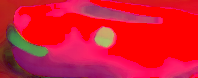
\includegraphics[width = 0.24\columnwidth]{Implementation/cv/m3.png}}
\subfigure{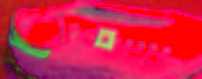
\includegraphics[width = 0.24\columnwidth]{Implementation/cv/b3.png}}

\subfigure{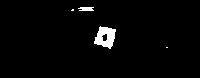
\includegraphics[width = 0.24\columnwidth]{Implementation/cv/bi4.png}}
\subfigure{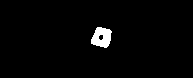
\includegraphics[width = 0.24\columnwidth]{Implementation/cv/g4.png}}
\subfigure{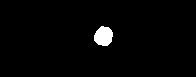
\includegraphics[width = 0.24\columnwidth]{Implementation/cv/m4.png}}
\subfigure{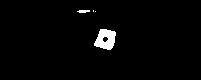
\includegraphics[width = 0.24\columnwidth]{Implementation/cv/b4.png}}

\subfigure{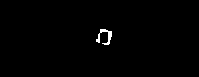
\includegraphics[width = 0.24\columnwidth]{Implementation/cv/bi5.png}}
\subfigure{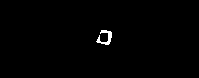
\includegraphics[width = 0.24\columnwidth]{Implementation/cv/g5.png}}
\subfigure{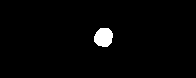
\includegraphics[width = 0.24\columnwidth]{Implementation/cv/m5.png}}
\subfigure{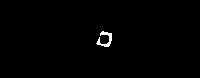
\includegraphics[width = 0.24\columnwidth]{Implementation/cv/b5.png}}

\subfigure[Bilateral filter]{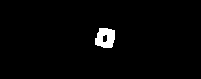
\includegraphics[width = 0.24\columnwidth]{Implementation/cv/bi6.png}}
\subfigure[Gaussian filter]{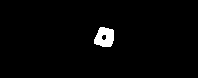
\includegraphics[width = 0.24\columnwidth]{Implementation/cv/g6.png}}
\subfigure[Median filter]{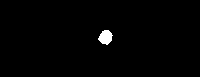
\includegraphics[width = 0.24\columnwidth]{Implementation/cv/m6.png}}
\subfigure[Normalized Box filter]{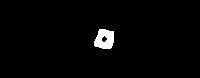
\includegraphics[width = 0.24\columnwidth]{Implementation/cv/b6.png}}
\caption{Image processing of extracted shoe region using ASUS Xtion camera. Each column uses one specific type of blurred filter. For each column, from top to bottom, each image is, in turn, the original image labeled with detected contour area, smoothed image after applying the linear filter, image of HSV color space of the smoothed image, mask for color 'blue', mask after $erode$ function, and the final mask after $dilate$ function}
\label{asusfilter}
\end{figure}

\begin{table}[H]
\centering
\resizebox{\columnwidth}{!}{
\begin{tabular}{||c||c|c||}
\hline
Waypoints & Left arm & Right arm \\ \hline\hline
$1$ & $[adl\_x, adl\_y, 0.3, -\frac{\pi}{4}, \pi, \pi]$ & $[adr\_x, adr\_y, 0.3, \frac{\pi}{4}, \pi, \pi]$ \\ \hline
$2$ & $[adl\_x, adl\_y, 0.1, -\frac{\pi}{4}, \pi, \pi]$ & $[adr\_x, adr\_y, 0.1, \frac{\pi}{4}, \pi, \pi]$ \\ \hline
$3$ & $[adll\_x, adll\_y, 0.1, -\frac{\pi}{4}, \pi, \pi]$ & $[adrr\_x, adrr\_y, 0.1, \frac{\pi}{4}, \pi, \pi]$ \\ \hline
$4$ & $[adl\_x, adl\_y, 0.1, -\frac{\pi}{4}, \pi, \pi]$ & $[adr\_x, adr\_y, 0.1, \frac{\pi}{4}, \pi, \pi]$ \\ \hline
$5$ & $[adl\_x, adl\_y, 0.3, -\frac{\pi}{4}, \pi, \pi]$ & $[adr\_x, adr\_y, 0.3, \frac{\pi}{4}, \pi, \pi]$ \\ \hline
\end{tabular}}
\caption{Shoe pose adjustment waypoints for both of YuMi's end-effectors}
\label{adjustwaypoints}
\end{table}